% !TeX root = ../main.tex

\section{Results}

Results will go here. I have some stuff on CarHMMs and HHMMs from STAT 548 but I need to put it together still.

\iffalse
\section{Case study- Fluking in Killer Whales}

\subsection{Data Collection and Preprocessing}

To demonstrate this methodology as applied to real-world data, the CarHMM was used to analyze dive data from a killer whale off the coast of British Columbia, Canada. The data was collected on September 2, 2019 from 12:49 pm to 6:06 pm and consists of depth and acceleration in three orthogonal directions. Observations were collected at a rate of 50 hertz. Tagging the killer whale caused anomalous behavior before 1:20 pm and after 6:00 pm, so observations in this time range were ignored. In addition, the tagging technology dropped data between 2:25pm and 2:37pm as well as between 4:07 and 5:07 pm, so any partially observed data within this time range were ignored as well. A killer whale ``dive" is considered to be any continuous chunk of data that occurs below 3.1 meters in depth and lasts for at least 10 seconds. Finally, for computational purposes, only dives that reached a depth of at least 20 meters were included in the analysis, resulting a total of 7 dives. Data preprocessing was done in part with the \textit{divebomb} package in Python \cite{Nunes:2018}.

The accelerometer recorded both the acceleration due to animal movement and due to gravity. The magnitude of acceleration due only to animal movement is the overall dynamic body acceleration (ODBA) of the killer whale and is known to be a good proxy of energy expenditure \cite{Gleiss:2011}. However, because accelerometer's orientation is unclear, the average acceleration for each component over the entire data collection window was subtracted out (to account for acceleration due to gravity) and the magnitude of the resulting vector was taken as an estimate for the ODBA. This ad-hoc method of removing the effect of gravity is highly prone to errors, especially because the killer whale changes its orientation often. Future work should use alternative methods to find the overall dynamic body acceleration of the whale.

Velocity in the vertical direction was estimated using a central finite difference of the depth data:
%
$$v_t = \frac{d_{t+1} - d_{t-1}}{2\Delta t} = \frac{d_{t+1} - d_{t-1}}{1/25} $$
%
where $v_t$ is measured in meters per second. Due to the high frequency of data collection, small observation errors in depth readings resulted in relatively large errors in the velocity data. To deal with this, the velocity data was smoothed using a Gaussian kernel function with a width of 51 data points ($\approx$ 1 second) ranging from -3 to 3 standard deviations. In particular, if $\phi$ is the pdf of a standard normal distribution, then:
%
\begin{align*}
v^{(smoothed)}_t &= \sum_{i=-25}^{25} \omega_i v_{t+i} \\
\omega_i &= \frac{\phi\left(\frac{3i}{25}\right)}{\sum_{j=-25}^{25}\phi\left(\frac{3j}{25}\right)}
\end{align*}
%
Figure (\ref{fig:smoothing}) shows the velocity data before and after smoothing.

\begin{figure}[h!]
	\centering
	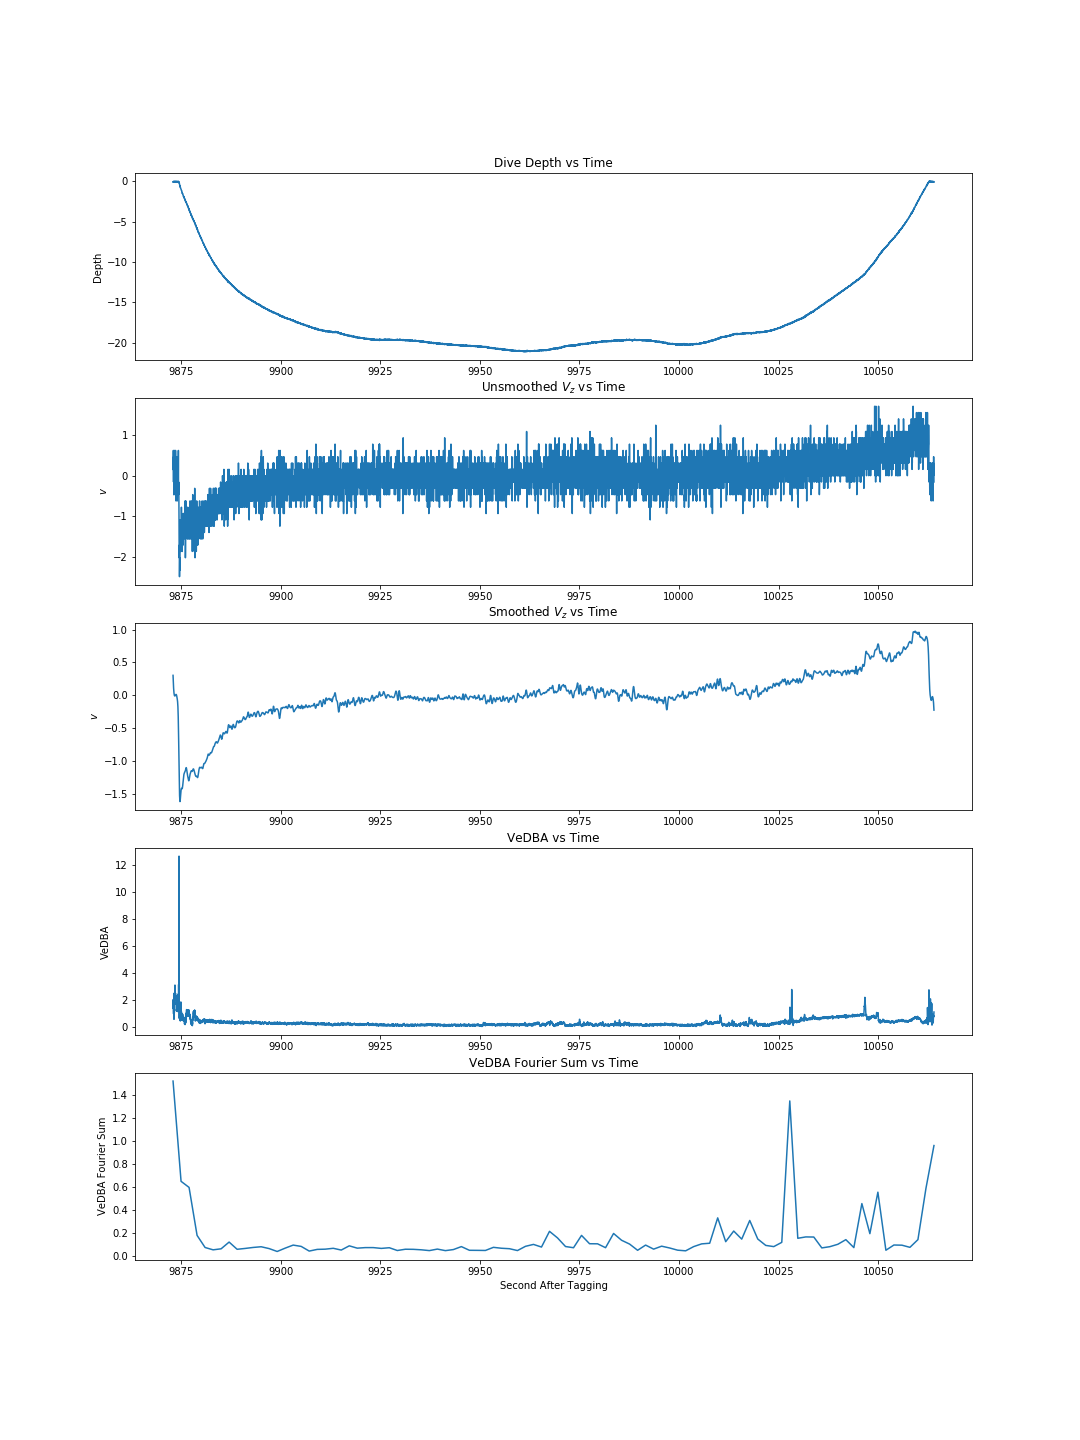
\includegraphics[height=7.5in]{../Plots/smoothed_v.png}
	\caption{From top to bottom: dive depth, unsmoothed vertical velocity, smoothed vertical velocity, ODBA, and the sum of low-frequency Fourier coefficeints of the ODBA for a randomly selected dive of a killer whale.}
	\label{fig:smoothing}
\end{figure}

Figure (\ref{fig:smoothing}) also shows the calculated ODBA as a function of time for one a specific dive. The acceleration exhibits sinusoidal behavior at several points in time which cannot be modeled using HMMs straightforwardly. As a result, the data was split into two-second intervals (100 data points each), and each interval was summarized by the Fourier transform of the ODBA and the velocity at the \textit{end} of the time interval. Velocity was taken at the end of the time interval because the behavior of the whale during the time interval has no impact on the velocity of the whale at the beginning of the time interval. Because velocity is highly correlated with the average acceleration within an interval, the mean was subtracted out of each ODBA time series before the Fourier transform was taken. To reduce the dimension of the ODBA Fourier transform, Fourier coefficients corresponding to frequencies less than or equal to 5 hertz were summed and frequencies above 5 hertz were ignored. One nice property of this process is that it reduces the number of data points by a factor of 100, which drastically speeds up parameter estimation. The optimal length of the time interval over which to take the Fourier transform is a tuning parameter that is difficult to find. An ideal time interval should be long enough give useful Fourier coefficients, but short enough to preserve as much information about the vertical velocity of the animal as possible.

\subsection{Lag Plot}

In order to find the appropriate HMM to model whale behavior, a lag plot was made for both velocity and the ODBA fourier sum. The results of doing so are shown in figure (\ref{fig:lag}). Unfortunately, the number of behavioral states is not clear from the lag plot, but it is clear that the velocity exhibits a large degree of autocorrelation. While the ODBA Fourier sum also exhibits some autocorrelation, the relationship is less strong, so autocorrelation was not incorporated in the ODBA Fourier sums emission distribution.

\begin{figure}[h!]
	\centering
	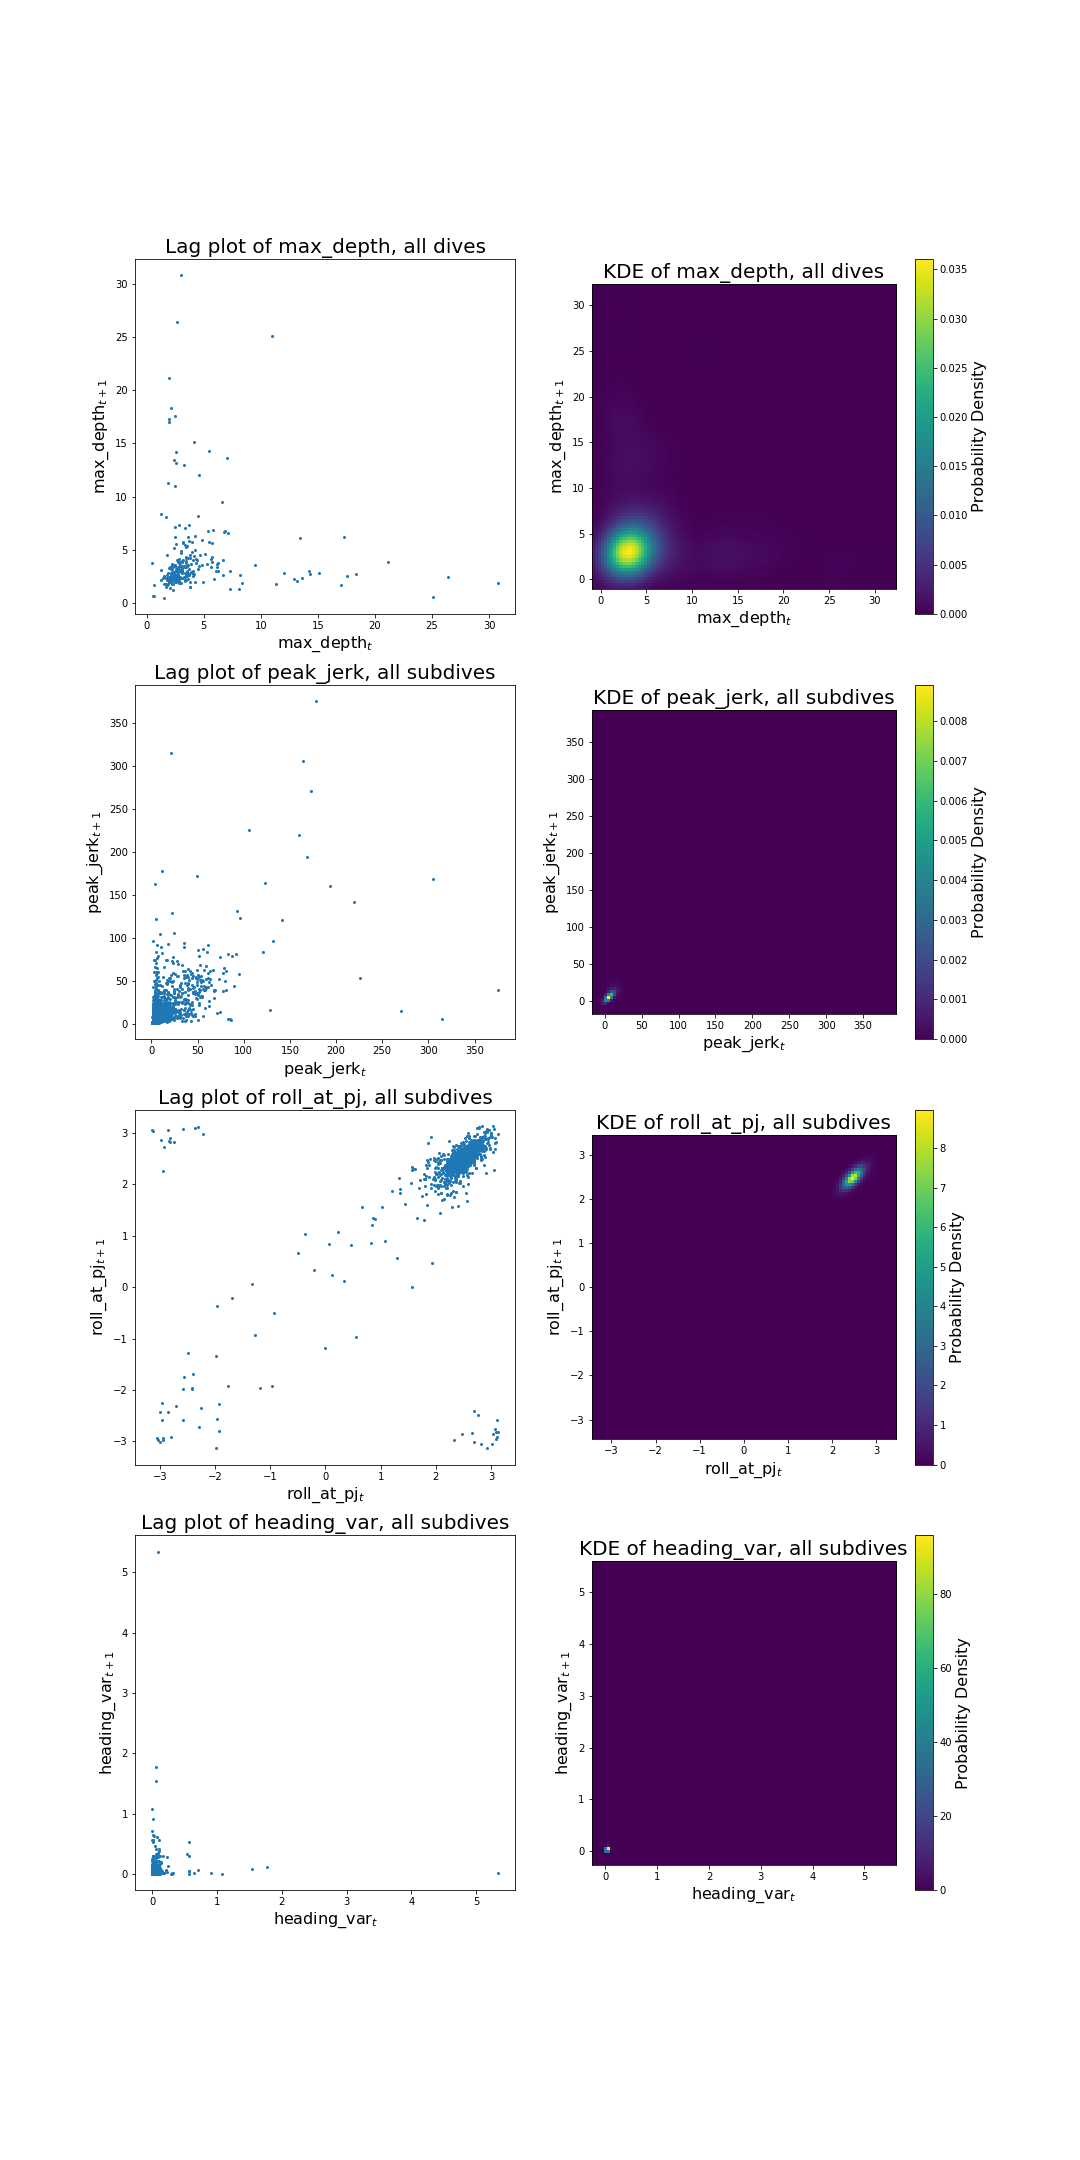
\includegraphics[height=5in]{../Plots/lagplot.png}
	\caption{Lag plot of vertical velocity and $\tilde a$ (left) and a the associated normal kernel density estimates (right)}
	\label{fig:lag}
\end{figure}

\subsection{CarHMM adapted to dive data}

Let $v_t$ represent the velocity in the $z-$direction (derived from depth data) at the end of time interval $t$ and $\tilde a_t$ represent the ODBA Fourier sum of interval $t$. The CarHMM was adapted to the dive data using the following model:

\begin{align*}
	v_{t} &\sim \mathcal{N}\left(\phi_{b_t} v_{t-1} + (1-\phi_{b_t}) \mu_{RL,b_t}, \sigma_{b_t}^2\right) \\
	%
	\tilde a_t &\sim \Gamma\left(\tilde \mu_{b_t}, \tilde \sigma^2_{b_t}\right)
\end{align*}

Note that the arguments in the gamma distribution above correspond to the mean and variance of the distribution, \textit{not} the standard scale and shape parameters. In total, 3 behavioral states were chosen for exploratory analysis as an attempt to capture behavioral states with very negative velocities, very positive velocities, and velocities close to zero. This results in a total of $3^2 + 4*3 = 21$ parameters, all of which were estimated using direct likelihood maximization.

\subsection{Results}

The parameters of the estimated emission distributions for each behavioral state are shown in table (\ref{table:emis_dist}) below. Each distribution is also plotted in figure (\ref{fig:emis_dist}). Note that the autocorrelation within the velocity sequence is not captured in figure (\ref{fig:emis_dist}), so it is important to refer to the estimated auto-correlation parameter $\hat \phi$ from table (\ref{table:emis_dist}) when considering the emission distributions shown in figure (\ref{fig:emis_dist}).
%
\begin{figure}[h!]
	\centering
	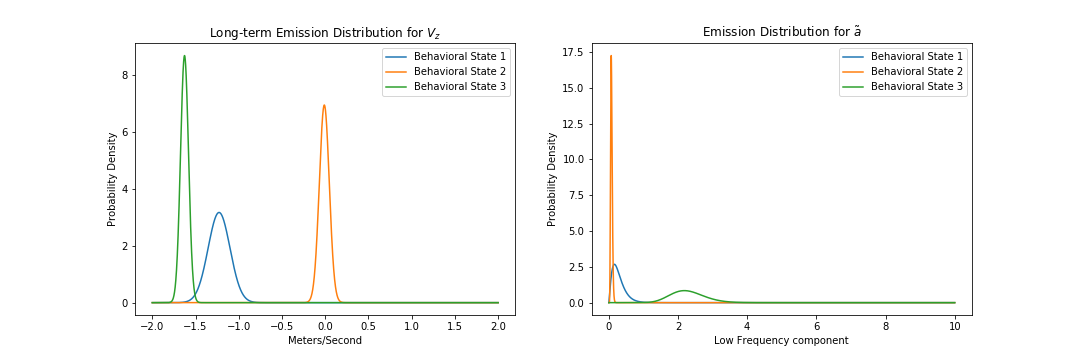
\includegraphics[height=2in]{../Plots/emis_dist.png}
	\caption{Estimated probability distributions for the long-term vertical velocity and $\tilde a$ in each behavioral state. Note that the distribution over vertical velocity does not take autocorrelation into account.}
	\label{fig:emis_dist}
\end{figure}
%
\begin{table}[h!]
	\centering
	\begin{tabular}{l|lll}
		& State 1 & State 2 & State 3 \\ \hline
		$\hat \mu_{RL}$        & 0.66    & 0.68    & 0.22    \\
		$\hat \sigma^2$        & 0.095   & 0.070   & 1.30    \\
		$\hat \phi$            & 0.88    & 0.99    & 0.03    \\ \hline
		$\hat \tilde \mu$      & 0.69    & 0.15    & 3.70    \\
		$\hat \tilde{\sigma^2}$ & 0.41    & 0.067   & 3.16   
	\end{tabular}
	\caption{Table of estimated parameters for probability distributions over $v$ and $\tilde a$ for each behavioral state}
	\label{table:emis_dist}
\end{table}
%
The estimated probability transition matrix and associated stationary distribution is shown below:

$$\hat \Gamma = \begin{pmatrix} 
0.7983 & 0.1618 & 0.0398 \\
0.0120 & 0.8796 & 0.0003 \\
0.2425 & 0.0049 & 0.7526
\end{pmatrix} \qquad \hat \delta = \begin{pmatrix} 0.4141 & 0.5020 & 0.0839 \end{pmatrix}$$

Finally, the Viterbi-decoded dive behavior within a randomly selected dive (deeper than 20 meters) is shown in figure (\ref{fig:viterbi}).

\newpage

\begin{figure}[h!]
	\centering
	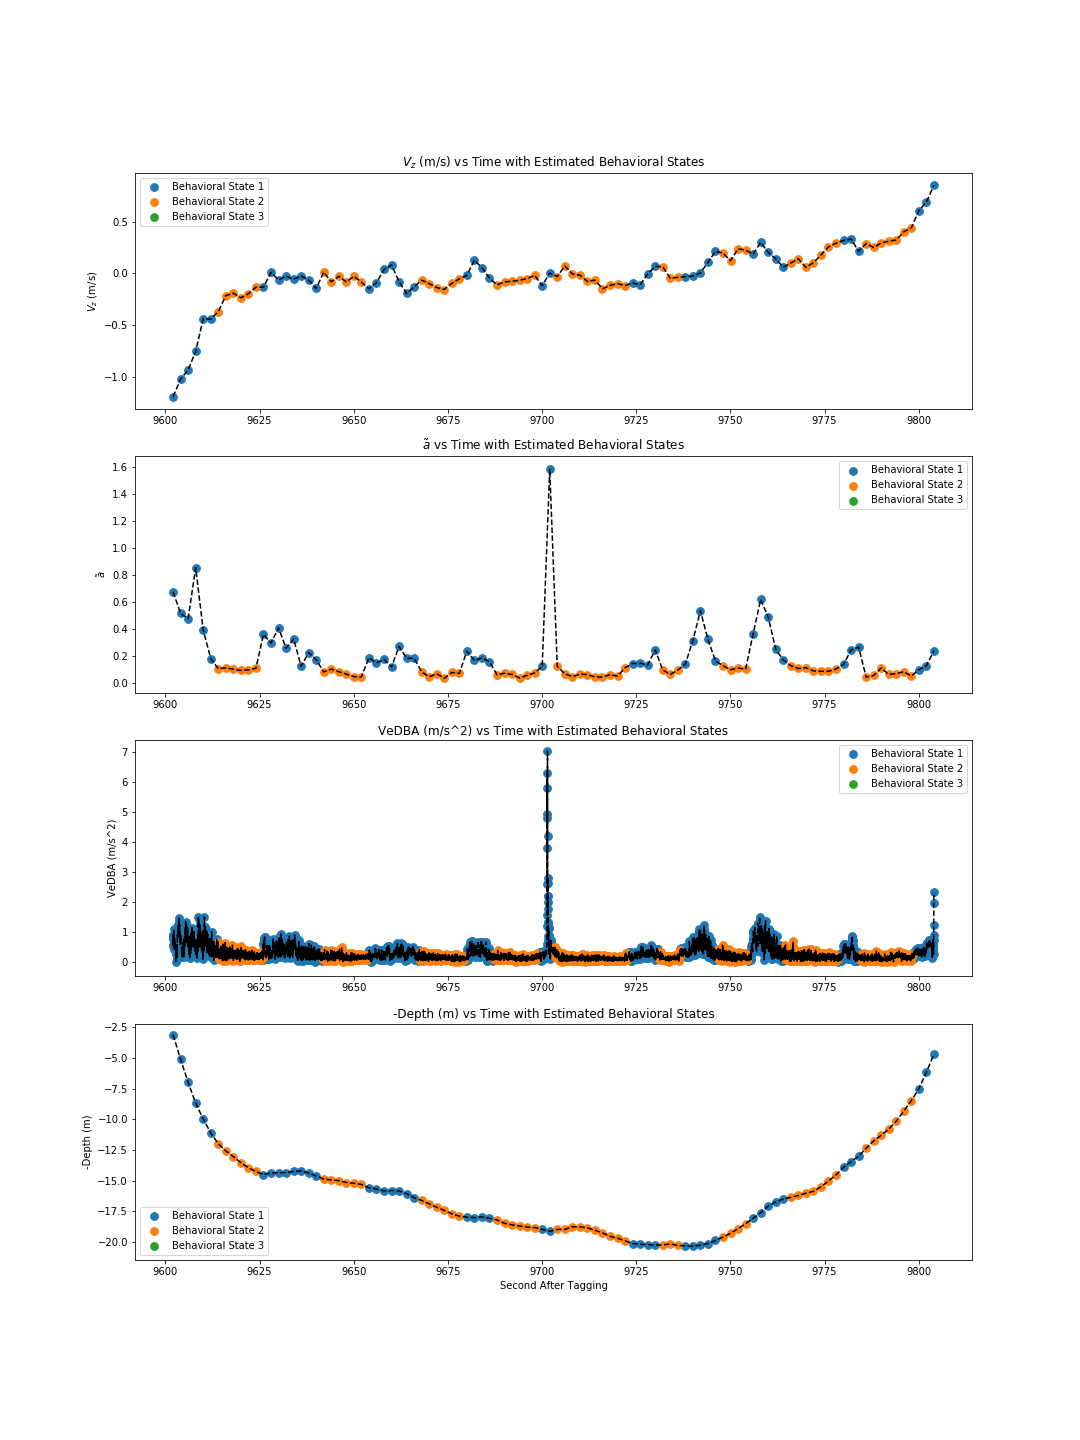
\includegraphics[height=8in]{../Plots/viterbi.png}
	\caption{Features of a particular killer whale dive and Viterbi-decoded estimates for the intra-dive behavioral states.}
	\label{fig:viterbi}
\end{figure}

\newpage

While the ecological meaning of these behavioral states is tenuous, we hypothesize the following interpretations. Roughly speaking, behavioral state 1 corresponds to mildly active swimming. The mean of $\tilde a$ in this state is larger than behavioral state 2, indicating more activity by the whale, but the autocorrleation term $\hat \phi$ is still very high, indicating that velocities don't change very much every two seconds. Behavioral state 2 corresponds to gliding or turning, where no active swimming is taking place. It is characterized by a low mean $\tilde a$ value and a very high autocorrelation term $\hat \phi$, both of which indicate little activity. Finally, behavioral state 3 represents sudden jerking or more vigorous and active swimming than behavioral state 1. This behavior is so rigorous that $\hat \phi$ drops almost to zero and $\hat \sigma^2$ subsequently rises significantly. In behavioral state 3, the velocity readings of the killer whale are essentially uncorrelated when recorded every two seconds.

\subsection{Future Work}

This analysis is largely exploratory with a purely heuristic approach to decide the number of behavioral states. Future work should repeat the analysis using several different values for the number of behavioral states. It is also important to validate these results by plotting psuedoresiduals and performing goodness-of-fit tests on the emission distributions.

Parameter estimation via likelihood maximization can be slow, especially with an observation rate of 50 hertz. If dives are modeled as uncorrelated batches of data, then using stochastic gradient ascent to maximize the likelihood may considerably speed up parameter estimation.

Finally, this work was run exclusively on dives deeper than 20 meters so that within-dive behaviors would be similar between dives. Future analysis could find a way to include a more heterogeneous set of dives using a framework such as the hierarchical hidden Markov model (HHMM) introduced by Leos-Barajas et al \cite{Barajas:2017}.

\fi